
\section{Project Overview}
We are developing a minimal 802.16-2009 OFDM Transmitter PHY.  This PHY
supports only QPSK-1/2 modulation-convolution rate. Additionally, any
components not relevant to unlicensed bands are omitted.  All optional items
are omitted.

This PHY requires the cooperation of a MAC layer implementation which is
compliant with the 802.16-2009 standard in order for the compliance
expectations (\autoref{sec:comply}) to be met.

\begin{wrapfigure}{r}{0.5\textwidth}
\begin{center}
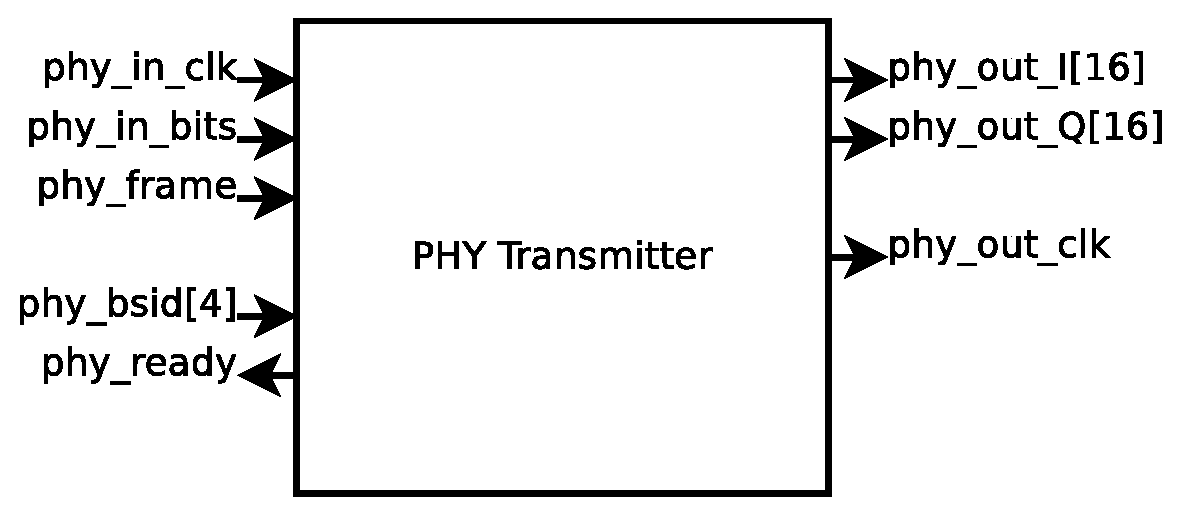
\includegraphics[width=0.48\textwidth]{t_block}
\caption{Overall Transmitter Interface}
\label{fiig:all-blockl}
\end{center}
\end{wrapfigure}

\begin{comment}
\todo[inline]{Derive the product from the needs}
\end{comment}

	\subsection{End Market Expectations}
	Currently IEEE 802.16, also known as ``WiMAX'', has seen little
	deployment in the United States and western Europe while being
	moderately deployed in Asian nations and Eastern European markets.
	To be useful in western areas, WiMAX has to effectively compete
	with both consumer owned Wifi hot-spots and the various cell phone
	networks. Given the impressively low cost of both cellular and Wifi
	(802.11) systems combined with the expectation that they work well
	in mobile devices, this physical layer (PHY) targets both
	simplicity (to reduce cost) and reduced power consumption.

	\subsection{Degree of standards compliance and scope limitations}
	\label{sec:comply}
	The 802.16 standard specifies multiple layers of a WiMAX device,
	including a ``Service-specific convergence
	sublayer''~\cite[section 5]{IEEE:802.16}, a MAC
	sublayer~\cite[section 6]{IEEE:802.16}, a Security
	sublayer~\cite[section 7]{IEEE:802.16}, and the Physical
	layer~\cite[section 8]{IEEE:802.16}. 
	
	The PHY, while being described within section 8 of the 802.16-2009
	document, is additionally subject to certain constraints and
	requirements stipulated within the other sections.  These sections
	where only utilized to the extent to which they apply to design of
	the PHY component.

	Applicable sections of \cite{IEEE:802.16}.
	\begin{itemize}
		\item Section 8.3 - OFDM description
		\item Section 8.3.3.4.1 - Data Modulation: implementation
			is not compliant with this section, only QPSK
			modulation is supported.
		\item 8.3.3.4.3 - Rate ID encodings: not compliant with
			this section, only the QPSK-1/2 rate ID is supported.
		\item 8.3.5.1.1 - DL subchannelization: Rate ID
	\end{itemize}